\chapter{Resultados e análises}\label{cap:resultados}

Neste capítulo serão apresentados resultados obtidos e os processos necessários para a obtenção dos mesmos. Como visto anteriormente no Capitulo 2,  uma das etapas
necessárias para a Análise de Sentimento é a classificação de polaridade dos \textit{tweets}. Durante a classificação, que gera o resultado da execução do Naive Bayes, foram utilizadas diversas formas de execução que serão apresentadas durante este capítulo.'

\section{Cenários e parâmetros de teste}\label{sec:cenarios}
Durante a execução dos testes para a análise de resultados o ambiente utilizado foi:
\begin{itemize}
	\item Sistema operacional: Linux Ubuntu
	\item Processador: Core i7
	\item Memória: 8GB
	\item Quantidade de \textit{tweets}: 141798
\end{itemize}


\section{Experimentos realizados e resultados}\label{sec:resultados}
O primeiro teste realizado para a classificação da base obteve o seguinte resultado:
\todo{Trazer tabela  1 pra ca}
\begin{table}[]
	\caption{1º teste}
	\label{teste-1}
	\resizebox{\textwidth}{!}{%
		\begin{tabular}{|l|l|r}
			\hline
			\multicolumn{3}{|c|}{1º Teste} \\ \hline
			\multicolumn{2}{|l|}{Bases usadas} & \multicolumn{1}{r|}{Tecnicas usadas} \\ \hline
			\multicolumn{2}{|c|}{Sentilex} & \multicolumn{1}{c|}{Stopwords} \\
			\multicolumn{2}{|c|}{PUC} & \multicolumn{1}{c|}{Stemming} \\ \cline{3-3} 
			\multicolumn{2}{|c|}{ReLi} &  \\ \hline
			\multicolumn{3}{|c|}{Resultado} \\ \hline
			\multicolumn{2}{|l|}{Positivo} & \multicolumn{1}{r|}{17350} \\ \hline
			\multicolumn{2}{|l|}{Negativo} & \multicolumn{1}{r|}{15517} \\ \hline
			\multicolumn{2}{|l|}{Neutro} & \multicolumn{1}{r|}{108931} \\ \hline
			\multicolumn{2}{|l|}{Tempo} & \multicolumn{1}{r|}{311.673 segundos} \\ \hline
		\end{tabular}%
	}
\end{table}

Analisando a tabela \ref{teste-1} é visto quais as bases utilizadas, nesse caso, Reli , PUC e Sentilex, as técnicas utilizadas nesse teste, \textit{Stopwords} e \textit{Stemming}, e o resultado que de 141798 \textit{tweets}, 17350 foram positivos, 15517 negativos e 108931 neutros, levando 311.673 segundos para executar o teste.
\todo{Adicionar imagem grafico 1}
\begin{figure}[!h]
	\centering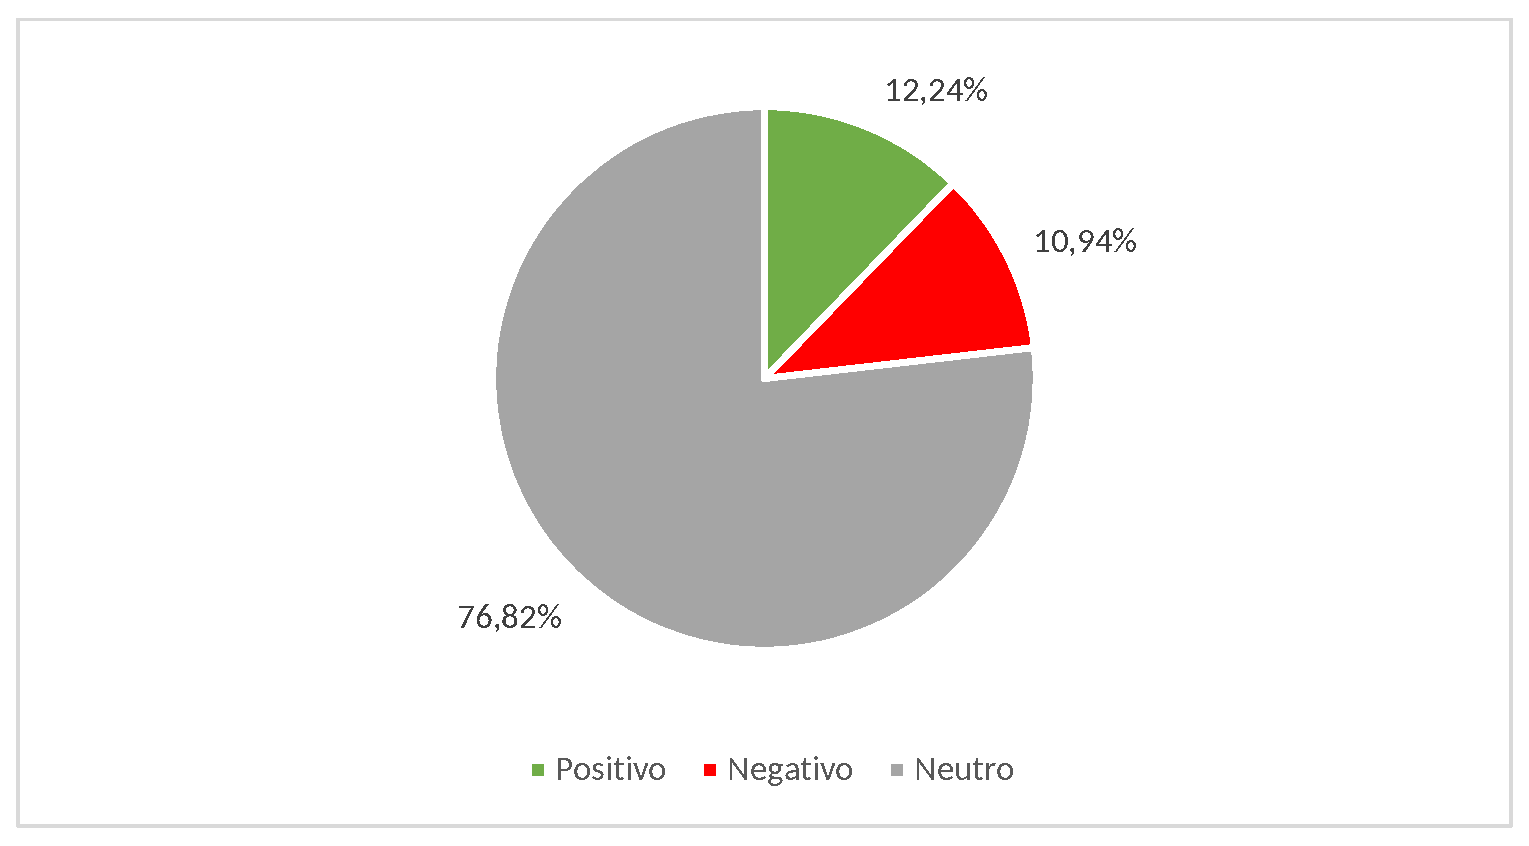
\epsfig{file=figuras/teste-1.eps, width=20cm}
	\caption{Quantidade de tweets separados por polaridade do teste 1. Fonte: Própria}
	\label{uni}
\end{figure}

Nota-se que a quantidade de \textit{tweets} neutros é muito alta, evidenciando que o modelo ainda tem dificuldade de definir a polaridade do texto. Com base nos resultados apresentados foram realizadas as seguintes mudanças visando diminuir a ocorrência de "neutros".
 
\todo{Tabela 2 aqui}

\begin{table}[]
	\caption{2º teste}
	\label{teste-2}
	\resizebox{\textwidth}{!}{%
		\begin{tabular}{|l|l|r}
			\hline
			\multicolumn{3}{|c|}{2º Teste} \\ \hline
			\multicolumn{2}{|l|}{Bases usadas} & \multicolumn{1}{r|}{Tecnicas usadas} \\ \hline
			\multicolumn{2}{|c|}{Sentilex-Stem} & \multicolumn{1}{c|}{Stopwords-Stem} \\
			\multicolumn{2}{|c|}{PUC-Stem} & \multicolumn{1}{c|}{Stemming} \\ \cline{3-3} 
			\multicolumn{2}{|c|}{ReLi} &  \\ \hline
			\multicolumn{3}{|c|}{Resultado} \\ \hline
			\multicolumn{2}{|l|}{Positivo} & \multicolumn{1}{r|}{49263} \\ \hline
			\multicolumn{2}{|l|}{Negativo} & \multicolumn{1}{r|}{35079} \\ \hline
			\multicolumn{2}{|l|}{Neutro} & \multicolumn{1}{r|}{57456} \\ \hline
			\multicolumn{2}{|l|}{Tempo} & \multicolumn{1}{r|}{397.48 segundos} \\ \hline
		\end{tabular}%
	}
\end{table}

No 2º teste visto na tabela \ref{teste-2} é visto que a quantidade de neutro diminuiu consideravelmente, apenas aplicando a técnica de \textit{stemming} nas bases de palavras
\todo{grafico 2}
\begin{figure}[!h]
	\centering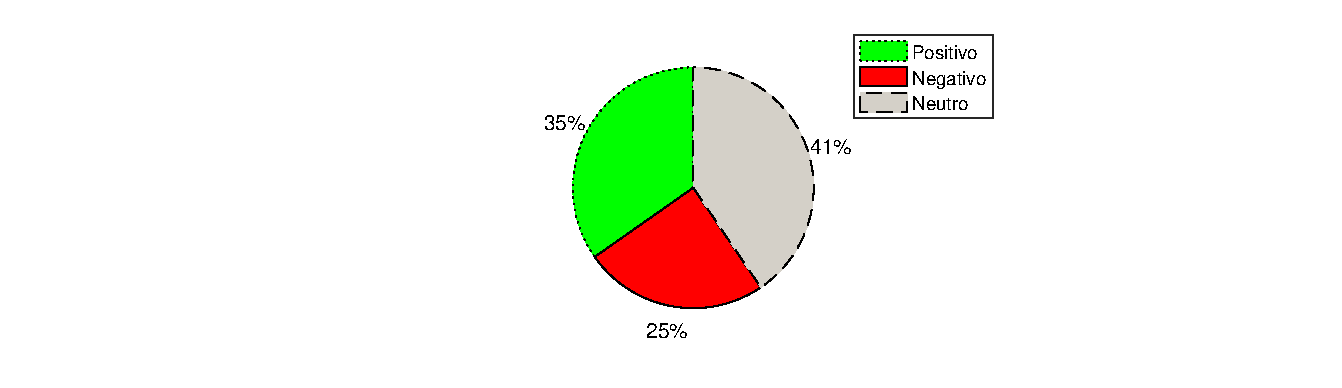
\epsfig{file=figuras/teste-2.eps, width=20cm}
	\caption{Quantidade de tweets separados por polaridade do teste 2. Fonte: Própria}
	\label{uni}
\end{figure}

Ainda buscando a diminuição de neutros foi criada uma base de palavras mas próxima do domínio que esse trabalho propõe que é o Oscar2016, essa base contem palavras relevantes a esse evento, gerando o seguinte resultado.
\todo{colocar tabela 3 aqui}

\begin{table}[]
	\caption{3º teste}
	\label{teste-3}
	\resizebox{\textwidth}{!}{%
		\begin{tabular}{|l|l|r|}
			\hline
			\multicolumn{3}{|c|}{3º Teste} \\ \hline
			\multicolumn{2}{|l|}{Bases usadas} & Técnicas usadas \\ \hline
			\multicolumn{2}{|c|}{Oscar2016} & \multicolumn{1}{c|}{\textit{Stopwords}} \\ \hline
			\multicolumn{3}{|c|}{Resultado} \\ \hline
			\multicolumn{2}{|l|}{Positivo} & 47450 \\ \hline
			\multicolumn{2}{|l|}{Negativo} & 7210 \\ \hline
			\multicolumn{2}{|l|}{Neutro} & 87138 \\ \hline
			\multicolumn{2}{|l|}{Tempo} & 709,126 segundos \\ \hline
		\end{tabular}%
	}
\end{table}

Analisando a tabela \ref{teste-3} é visto que apenas uma base mais especializada no domínio não consegue diminuir a quantidade de neutros e ainda aumenta o tempo para a execução dos testes.
\todo{grafico 3}
\begin{figure}[!h]
	\centering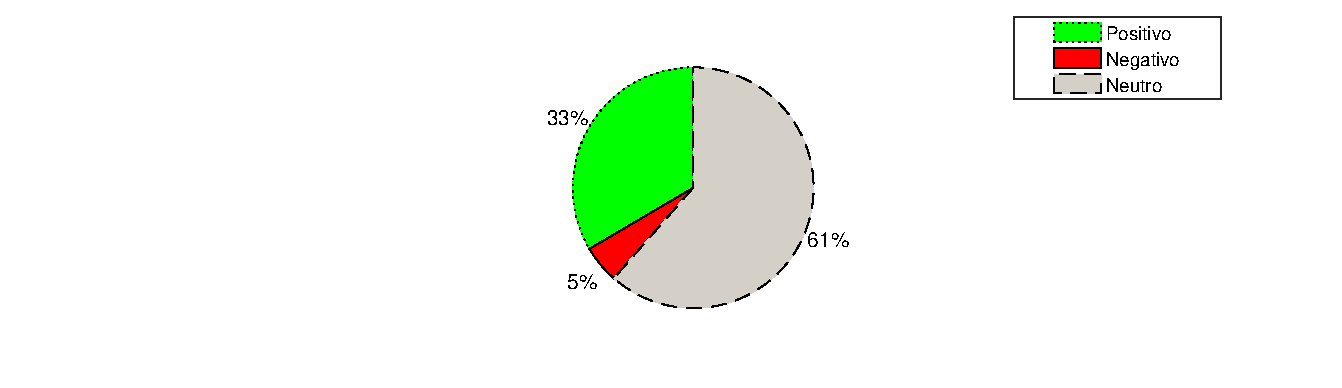
\epsfig{file=figuras/teste-3.eps, width=20cm}
	\caption{Quantidade de tweets separados por polaridade do teste 3. Fonte: Própria}
	\label{uni}
\end{figure}

No 4º teste foi adicionada o base criada, Oscar2016, com as bases genéricas, gerando o seguinte resultado:
\begin{table}[]
	\caption{4º teste}
	\label{teste-4}
	\resizebox{\textwidth}{!}{%
		\begin{tabular}{|c|l|r}
			\hline
			\multicolumn{3}{|c|}{4º Teste} \\ \hline
			\multicolumn{2}{|l|}{Bases usadas} & \multicolumn{1}{r|}{Técnicas usadas} \\ \hline
			\multicolumn{2}{|c|}{Oscar2016} & \multicolumn{1}{c|}{Stopwords} \\
			\multicolumn{2}{|c|}{SentiLex} & \multicolumn{1}{c|}{Stemming} \\ \cline{3-3} 
			\multicolumn{2}{|c|}{PUC} & \multicolumn{1}{c}{} \\
			\multicolumn{2}{|c|}{ReLi} & \multicolumn{1}{c}{} \\ \hline
			\multicolumn{3}{|c|}{Resultado} \\ \hline
			\multicolumn{2}{|l|}{Positivo} & \multicolumn{1}{r|}{69070} \\ \hline
			\multicolumn{2}{|l|}{Negativo} & \multicolumn{1}{r|}{33461} \\ \hline
			\multicolumn{2}{|l|}{Neutro} & \multicolumn{1}{r|}{39267} \\ \hline
			\multicolumn{2}{|l|}{Tempo} & \multicolumn{1}{r|}{650.97 segundos} \\ \hline
		\end{tabular}%
	}
\end{table}

Analisando a tabela \ref{teste-4} é visto que nesse teste foi obtida a maior diminuição de neutros, mas com um tempo de processamento um pouco maior.
\todo{Adicionar grafico 4}
\begin{figure}[!h]
	\centering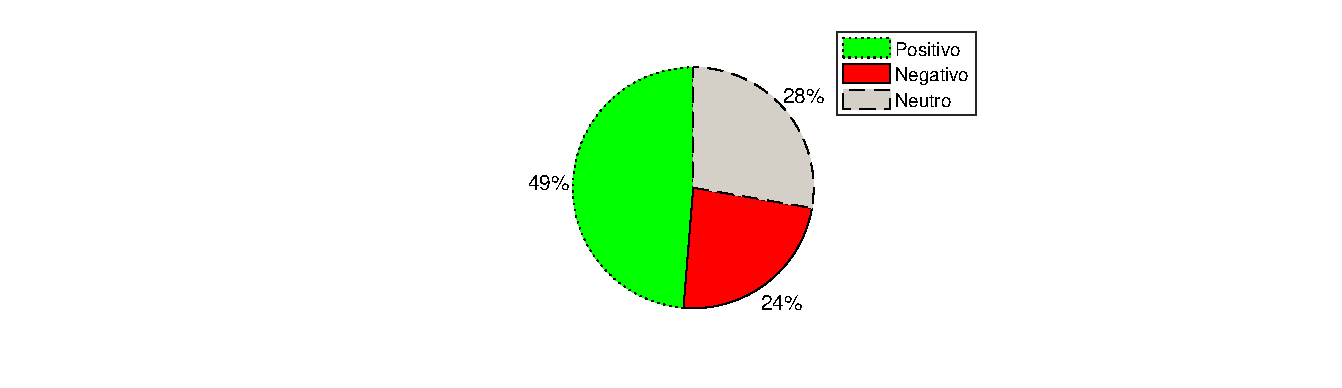
\epsfig{file=figuras/teste-4.eps, width=20cm}
	\caption{Quantidade de tweets separados por polaridade do teste 4. Fonte: Própria}
	\label{uni}
\end{figure}
Segue abaixo um comparativo dos testes.

\begin{table}[]
	\caption{Comparando testes}
	\label{teste-comp}
	\resizebox{\textwidth}{!}{%
		\begin{tabular}{l|l|c|l|l|}
			\cline{2-5}
			\multicolumn{1}{c|}{} & \multicolumn{1}{c|}{Teste 1} & Teste 2 & \multicolumn{1}{c|}{Teste 3} & \multicolumn{1}{c|}{Teste 4} \\ \hline
			\multicolumn{1}{|l|}{Positivo} & 15517 & \multicolumn{1}{r|}{49263} & 47450 & 69070 \\ \hline
			\multicolumn{1}{|l|}{Negativo} & 17350 & 35079 & 7210 & 33461 \\ \hline
			\multicolumn{1}{|l|}{Neutro} & 108931 & \multicolumn{1}{l|}{57456} & 87138 & 39267 \\ \hline
			\multicolumn{1}{|l|}{Tempo (s)} & \multicolumn{1}{c|}{311.673} & 397.48 & 709.129 & 650.97 \\ \hline
		\end{tabular}%
	}
\end{table}
